\documentclass[12pt]{article}

\usepackage[pdftex]{graphicx}
\usepackage{hyperref}
\usepackage{listings}
\lstset{language=C}
\hypersetup{colorlinks=true, citecolor=blue, urlcolor=blue}
\usepackage[margin=1in]{geometry}

\usepackage{fancyhdr}
\pagestyle{fancy}

%\usepackage{mathptmx} 
%\linespread{1.05}
%\usepackage[T1]{fontenc}

\setcounter{secnumdepth}{-1} 
\setlength{\headheight}{15pt}



\begin{document}
\fancyhead[LO]{RAS UT Austin \today}


\begin{center}
{\Huge 2012 IEEE Region V Robotics Technical Paper}\\[\baselineskip]
\end{center}
{\large\itshape IEEE Robotics and Automation Society University of Texas at Austin}\\[\baselineskip]
\today 

\section{Introduction}
\subsection{Aims and Objectives}
The challenge was to harvest energy from three different energy sources and deliver to an electrochemical device (i.e. the flag) to measure the amount of energy transmitted. The robot needed to capture energy from at least two of three sources (either wind, light, or electric) and transfer the energy to a flag mechanism. All sources and the flag mechanism were at various corners of the playing field. The light source was a 50 Watt Halogen MR16 GU10 Base Flood Light Bulb powered by a 115 V, 60 Hz outlet. The electric source was a 5 V Thevenin source with 24 Ohm Thevenin resistance. The wind source was a Style by Revlon 1875 Watt Dryer set to high and cold shot. Once the robot harvested the energy from the sources, it would power a gear motor (Part No. 1094, Pololu Robotics) to raise and lower the flag. 



%\subsection{Objectives}
%\begin{itemize}
%	\item Capture energy from at least two of three sources (either wind, light, or electric)
%	\item Transfer stored energy to the flag mechanism
%\end{itemize}
%\subsection{Project Restrictions}
%\begin{itemize}
%	\item The playing field was a 8 foot by 8 foot medium-density fibreboard (MDF) surface divided into four %quadrants. Each quadrant consisted of an energy source in the corner. 
%\end{itemize}

%\begin{figure}[htbp] %  figure placement: here, top, bottom, or page
%  \centering
%  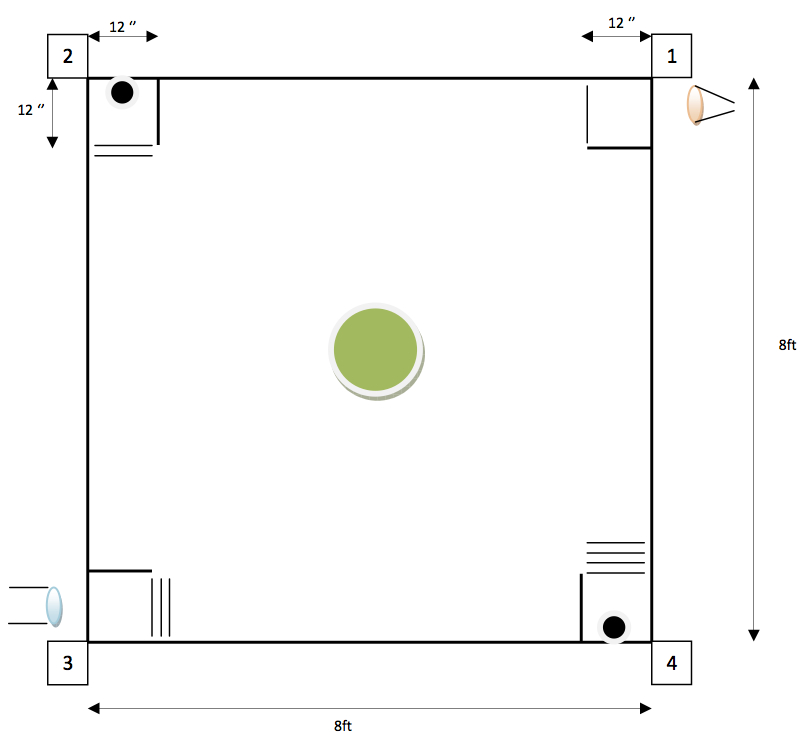
\includegraphics[width=3in]{Robotics2012PlayingField} 
%   \caption{Playing Field Diagram}
%  \label{fig:playing field}
%\end{figure}

%\begin{itemize}
%	\item Energy Sources
%		\begin{enumerate}
%			\item Light Source (Quadrant 1): 50 Watt Halogen MR16 GU10 Base Flood Light Bulb powered by 115 V, 60 Hz Outlet. The center of the bulb was 6 inches above the playing field. The circular surface of the bulb was 6 inches away from the inside surface of the perimeter. 
%			\item Electric Source (Quadrant 2): 5 V Thevenin source with 24 Ohm Thevenin resistance. Source is housed in a 3 inch PVC cap. Electrical contacts were 0.5 inch wide thin-metal strips. The top strip was positive. 
%			\item Wind Source (Quadrant 3): Style by Revlon 1875 Watt Dryer. Hair Dryer was set on High and Cold Shot permanently depressed. The center of the opening duct was 6 inches above the playing field. The circular surface of the dryer was 6 inches away from the inside surface of the perimeter. 
%		\end{enumerate} 
%\end{itemize}
%\begin{itemize}
%	\item Delivery Flag (Quadrant 4): Essentially, a gear motor (Part No. 1094, Pololu Robotics) raises and lowers a small block. There will be a zener diode (approx. 6 V) in parallel with the motor to prevent motor damage. TO BE DONE. 
%\end{itemize}
%\begin{figure}[htbp] %  figure placement: here, top, bottom, or page
%   \centering
%  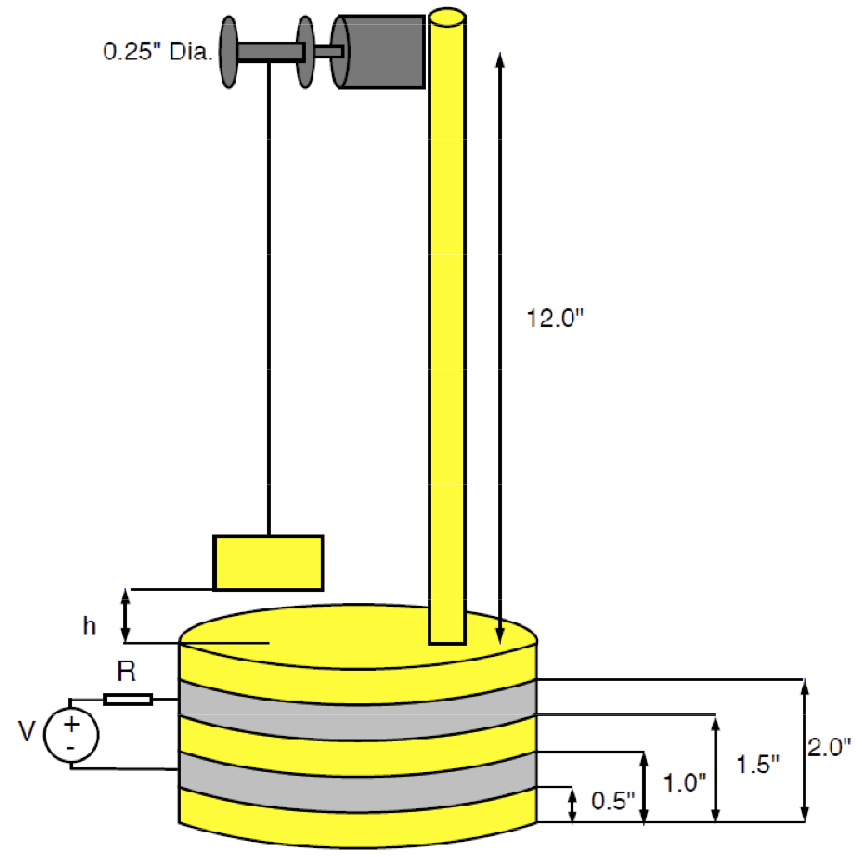
\includegraphics[width=3in]{Robotics2012Flag} 
%   \caption{Flag Mechanism}
%   \label{fig:flagmechanism}
%\end{figure}
%\begin{itemize}
%	\item Starting Tree (Center): The robot will start from the center of the field. In the center is a tree inside a five %gallon bucket. Some part of the robot must touch the outside diameter of the bucket as its starting position. 
%	\item Source Switching. Sources will be turned on and off throughout the round. 
%	\item Robot Limitations
%		\begin {enumerate}
%			\item The robot could not cross the perimeter to harvest light energy or wind energy. 
%			\item Maximum dimensions are 1 foot by 1 foot by 1 foot. 
%		\end {enumerate}
%\end{itemize}

		
		
\section{Modules}

\subsection{Printed Circuit Board}
The Stellaris Arm LM 35811 served as the main processing unit for the system. Communication components include a USB to JTAG, a Serial Peripheral Interface Bus, and an Inter-Integrated Circuit bus. There are also ports for Analog Input and Digital I/O. A 8.4 V battery supplies voltage to the circuit board. 

%\begin{figure}[htbp] %  figure placement: here, top, bottom, or page
%  \centering
%  \includegraphics[scale=0.4]{RASBoardCircuit1} 
%   \caption{USB to JTAG and Serial}
%   \label{fig:MicroController1}
%\end{figure}

%\begin{figure}[htbp] %  figure placement: here, top, bottom, or page
%   \centering
%   \includegraphics[scale=0.4]{RASBoardCircuit2} 
%   \caption{H-Bridges and Encoders}
%   \label{fig:MicroController2}
%\end{figure}

%\begin{figure}[htbp] %  figure placement: here, top, bottom, or page
%   \centering
%   \includegraphics[scale=0.4]{RASBoardCircuit3} 
%   \caption{Power Circuit, Reset Switch, MCU}
%   \label{fig:MicroController3}
%\end{figure}

%\begin{figure}[htbp] %  figure placement: here, top, bottom, or page
%   \centering
%   \includegraphics[scale=0.4]{RASBoardCircuit4} 
%   \caption{Analog Input, Digital I/O, SPI and I2C}
%   \label{fig:MicroController4}
%\end{figure}

\subsection{IR Sensor/Wall following}
In this robot there are 6 Infrared Sensors (Sharp 2D120X) around the peripheral of the robot base. They produce an analog output between 3.1 V at 4 cm and 0.3 V at 30 cm. The sensors are used in conjunction with wall-following code to help determine the direction the robot should be moving. 


\subsection{Charging and Discharging} There are three 1 F capacitors to store energy from the various sources. When charging, the capacitors will be placed in parallel and when discharging, will be placed in series. Each capacitor will be charged to 2 V for a total of 6 V when in series. There are also four relays (Aromat/Panasonic HC4-HL-DC24V)  that operate at 12 V. Mosfets are used to switch the relays with 4 V. When the mosfets are not conducting, there is an open circuit and the relays are off. When the mosfets are conducting, the circuit is complete, and the relays turn on. The first relay is a multiplexer to select between the three input sources (charging) and the output (discharging). The second relay guarantees that only source is going into the capacitors. The third relay serves as a disconnector and backup to the charging device. A digital zero corresponds to normal mode and a digital one corresponds to disconnecting the output to the capacitor. The fourth relay changes the three capacitors from series to parallel. Off corresponds to a parallel configuration and On corresponds to a series configuration.There will be two relays for each subsequent capacitor (capacitor no. 2 and capacitor no. 3). The relays can be either on or off (different connections). See Figure 1.  

%{
%\begin{figure}[htbp] %  figure placement: here, top, bottom, or page
%  \centering
%  \includegraphics[scale=0.7]{CapacitorsRelays} 
%  \caption{Capacitors and Relays}
%  \label{fig:CapacitorsRelays}
%  \end{figure}
% }




\subsection{Motors and Movement}
We used two motors, one on the left end and the other on the right end of the robot. The two motors use a servomechanism with two quadrature encoders (incremental rotary encoders) to provide feedback about the direction of the rotating shaft. The motors have built in optical encoders separated by optical ticks that count the number of ticks between when light is sensed and when it is not sensed.The potentiometer in the servo determines what angle the robot is moving, what angle it will be moving at, and also corrects the power to the motor. A pulse (50 Hz) to the servo controls the angle of the servo (0 -90, 90 -180) and motor-speed through a h-bridge circuit. The duty cycle (percentage on/ percentage off) is around 0.5 ms - 2.5 ms. A caster is attached to the middle of the robot to support the robot frame and to help maneuver. 

\subsection{Solar Panels}
To maximize the current, we placed six panels in parallel in two rows. We expect the voltage across each panel to be approximately 4 V and the resultant maximum voltage to be 8 V. In addition, there are two servos (Hitec HS-300) to rotate it into the optimal position to obtain solar energy. When the solar panels are not being used, they will be positioned in parallel with the robot base so that the other modules may be used. See Figure 2. 


\subsection{Fans}fff

\subsection{Electrical Source}ffff

\subsection{Body/Chassis}ffff

\subsection{Program}
We used Keil uVision IDE to develop the software for the micro controller. 

\lstinputlisting{}


{
\begin{figure}[htbp]
  \centering
  \includegraphics[width=\textwidth,height=\dimexpr\textheight-2\baselineskip\relax,keepaspectratio]{Relays}
  %\includegraphics[width=\textwidth,height=\textheight,keepaspectratio]{Relays}
  %\includegraphics[scale=0.5]{Relays}
  \caption{Charging and Discharging Module}
  \label{fig:CapacitorsRelays}
\end{figure}
  }
  
  {
\begin{figure}[htbp] %  figure placement: here, top, bottom, or page
  \centering
  \includegraphics[scale=0.5]{SolarPanels} 
  \caption{Solar Panels}
   \label{fig:SolarPanels}
\end{figure}
}

\subsection{References}
[1]. Sharp 2D120X http://www.phidgets.com/documentation/Phidgets/3520Datasheet.pdf (accessed April 20, 2012)
\newline
[2]. Panasonic HC4 HL DC24V http://datasheet.octopart.com/HC4-HL-DC24V-Panasonic-datasheet-109869.pdf (accessed April 20, 2012)
\end{document}

